\hypertarget{metodología}{%
  \section{Metodología}\label{Metodología}}

\subsection{Enfoque de la investigación}

En esta investigación se empleará un enfoque cuantitativo, con el objetivo de analizar de manera objetiva y cuantificable
la relación entre la resolución de la guía de programación y el éxito académico en el curso de Introducción a la
Programación de la Universidad Andrés Bello.

\subsection{Diseño de investigación}

En este estudio, se empleará la metodología KDD (Knowledge Discovery in Databases, descubrimiento de conocimiento en bases de datos) para llevar a cabo el análisis de los datos. El proceso de KDD consta de varias etapas fundamentales que nos permitirán obtener conocimientos relevantes a partir de los datos recopilados. Estas etapas incluyen:

\textbf{Selección de datos}: En esta etapa, se identificarán y seleccionarán los datos relevantes para el estudio. En nuestro caso, utilizaremos el conjunto de datos "dataset a 2021" que contiene información sobre los resultados de la guía de programación y el rendimiento en la primera evaluación del curso de Introducción a la Programación en la Universidad Andrés Bello en el año 2021.

\textbf{Preparación de datos}: En esta etapa, se realizarán las transformaciones necesarias en los datos seleccionados para garantizar su calidad y adecuación al análisis. Esto puede incluir la limpieza de datos, la eliminación de valores atípicos o faltantes, y la normalización de variables, entre otros procesos.

\textbf{Minería de datos}: En esta etapa, se aplicarán técnicas de minería de datos para descubrir patrones, relaciones y tendencias ocultas en los datos. Utilizaremos técnicas estadísticas y algoritmos de aprendizaje automático para explorar la relación entre la resolución de la guía de programación, el éxito académico y el programa de estudio de los estudiantes.

\textbf{Evaluación de resultados}: En esta etapa, se evaluarán los resultados obtenidos a través de la minería de datos. Se analizarán los patrones identificados, se medirá su significancia estadística y se evaluará su relevancia para los objetivos de la investigación.

\textbf{Interpretación de hallazgos}: Finalmente, en esta etapa, se interpretarán los hallazgos obtenidos a partir del análisis de los datos. Se examinarán los resultados en el contexto de la pregunta de investigación planteada y se realizarán inferencias y conclusiones basadas en los patrones y relaciones descubiertos.

\begin{figure}[H]
  \centering
  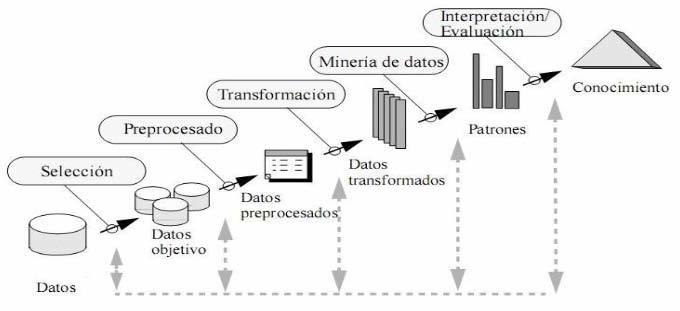
\includegraphics[width=4.06111in,height=2.68611in]{img/KDD.png}
  \caption{Flujo gráfico KDD}
  \label{fig:flujo_kdd}
\end{figure}

Al seguir la metodología KDD, nos aseguraremos de seguir un enfoque sistemático y riguroso para el análisis de los datos recopilados, lo que nos permitirá obtener conocimientos significativos y relevantes relacionados con la resolución de la guía de programación, el éxito académico y la deserción estudiantil en el curso de Introducción a la Programación en la Universidad Andrés Bello.


\subsection{Descripción de la base de datos}

En esta investigación, se utiliza un conjunto de datos que registra a los estudiantes que tomaron el
curso de Introducción a la Programación en la Universidad Andrés Bello durante el año 2021.
Estos datos incluyen información sobre el rendimiento de los estudiantes en la resolución de la guía de apoyo para la primera evaluación.

La base de datos cuenta con un total de 839 registros que registran información detallada de los
estudiantes, y se compone de 75 columnas que contienen diversas variables relacionadas con el curso
y el desempeño de los estudiantes.

\subsection{Recopilación de datos}

Para llevar a cabo este estudio, se cuenta con el conjunto de datos denominado "dataset a 2021", que contiene la información necesaria sobre los
resultados de la guía de programación y el rendimiento en la primera evaluación del curso de Introducción a la Programación en el año 2021.


\subsection{Análisis de datos}

Una vez recopilados los datos, se realizará un análisis descriptivo para examinar la distribución de los resultados en la guía de programación y la primera evaluación. Además, se llevará a cabo un análisis de correlación entre las variables mencionadas anteriormente para identificar posibles
relaciones y patrones significativos.

\subsection{Aplicación de XAI y SHAP}

En esta investigación, se planea utilizar técnicas de XAI (Explicabilidad de la Inteligencia Artificial) y SHAP (Shapley Additive Explanations) para comprender mejor el impacto de la resolución de la guía de programación en el éxito académico en el curso de Introducción a la Programación de la Universidad Andrés Bello.

XAI proporciona métodos y herramientas para interpretar y explicar las decisiones tomadas por los modelos de inteligencia artificial. En este estudio, se utilizará XAI para analizar los factores que influyen en la relación entre la resolución de la guía de programación y el éxito académico. Esto permitirá identificar las características o patrones específicos en las respuestas de los estudiantes que están relacionados con un mayor rendimiento académico.

Además, se empleará SHAP como una técnica de atribución para evaluar la importancia relativa de las diferentes características de la guía de programación en la predicción del éxito académico. SHAP proporciona una medida cuantitativa de la contribución de cada variable en la toma de decisiones del modelo. Mediante el uso de SHAP, se podrá determinar qué aspectos de la resolución de la guía de programación tienen un mayor impacto en el rendimiento académico de los estudiantes.

Al combinar el enfoque cuantitativo con XAI y SHAP, esta investigación pretende brindar una comprensión más profunda y detallada de la relación entre la resolución de la guía de programación y el éxito académico. Estas técnicas permitirán identificar los aspectos críticos que pueden influir en el rendimiento de los estudiantes y proporcionar información valiosa para mejorar los procesos de enseñanza y aprendizaje en el curso de Introducción a la Programación.

\subsection{Modelos de Clasificación}

En esta sección, se presentan los modelos de clasificación que serán utilizados en el estudio. Se explicará cada modelo en su respectiva subsubsección, incluyendo una descripción general y sus características principales.

\subsubsection{DecisionTreeClassifier}

El DecisionTreeClassifier es un modelo de clasificación basado en árboles de decisión. Este modelo construye un árbol en el que cada nodo representa una característica y cada rama representa una posible decisión o resultado. El árbol se construye de manera que las instancias se clasifiquen en las hojas del árbol, siguiendo una serie de reglas de decisión basadas en las características de los datos. El DecisionTreeClassifier es conocido por su capacidad para capturar relaciones no lineales y su interpretabilidad.

\subsubsection{LogisticRegression}

La LogisticRegression es un modelo de clasificación que se basa en el concepto de regresión logística. Este modelo utiliza la función logística para modelar la relación entre las variables independientes y la probabilidad de pertenecer a una clase específica. La regresión logística es especialmente útil en problemas de clasificación binaria, donde se desea predecir la probabilidad de pertenecer a una de las dos clases. Es un modelo lineal que puede manejar características numéricas y categóricas.

\subsubsection{RandomForestClassifier}

El RandomForestClassifier es un modelo de clasificación que combina múltiples árboles de decisión en un conjunto o "bosque". Cada árbol en el conjunto se entrena en una muestra aleatoria de los datos y produce una predicción independiente. Luego, se utiliza la mayoría de votos o la media de las predicciones individuales para obtener la predicción final. El RandomForestClassifier es conocido por su capacidad para manejar características irrelevantes y su resistencia al sobreajuste.

\subsubsection{XGBClassifier}

El XGBClassifier, abreviatura de Extreme Gradient Boosting Classifier, es un modelo de clasificación basado en el algoritmo de Gradient Boosting. Este modelo construye un conjunto de árboles de decisión de manera secuencial, donde cada árbol se ajusta a los errores residuales del árbol anterior. El XGBClassifier utiliza técnicas avanzadas, como el muestreo de características y la regularización, para mejorar el rendimiento y evitar el sobreajuste. Es conocido por su velocidad y precisión en problemas de clasificación.

\subsection{Modelos de Regresión}

En esta sección, se presentan los modelos de regresión que serán utilizados en el estudio. Se explicará cada modelo en su respectiva subsubsección, incluyendo una descripción general y sus características principales.

\subsubsection{LinearRegression}

La LinearRegression es un modelo de regresión que busca establecer una relación lineal entre las variables independientes y la variable dependiente. Este modelo asume que existe una relación lineal y busca encontrar los coeficientes que minimicen la suma de los errores cuadráticos entre las predicciones y los valores reales. La LinearRegression es conocida por su simplicidad y facilidad de interpretación.

\subsubsection{DecisionTreeRegressor}

El DecisionTreeRegressor es un modelo de regresión basado en árboles de decisión. Este modelo construye un árbol en el que cada nodo representa una característica y cada rama representa una posible decisión o resultado. El árbol se construye de manera que las instancias se asignen a las hojas del árbol, siguiendo una serie de reglas de decisión basadas en las características de los datos. El DecisionTreeRegressor es conocido por su capacidad para capturar relaciones no lineales en los datos de regresión.

\subsubsection{KNeighborsRegressor}

El KNeighborsRegressor es un modelo de regresión basado en el algoritmo de los k vecinos más cercanos. Este modelo asigna un valor de regresión a una instancia basándose en los valores de las k instancias más cercanas en el espacio de características. La predicción se realiza tomando la media (en el caso de regresión) de los valores de las k instancias más cercanas. El KNeighborsRegressor es conocido por su simplicidad y flexibilidad en problemas de regresión.

En el siguiente capítulo, se detallará la metodología utilizada para comparar el rendimiento de estos modelos en los problemas de clasificación y regresión.



\subsection{Comparación de Métricas entre Modelos de Clasificación}

En esta sección, se presentan las métricas utilizadas para comparar el rendimiento de diferentes modelos en el contexto del problema de clasificación. Se consideraron los siguientes modelos: DecisionTreeClassifier, LogisticRegression, RandomForestClassifier y XGBClassifier. A continuación, se describen las métricas utilizadas:

\subsubsection{Accuracy}
El accuracy, o precisión, es una métrica que mide la proporción de instancias clasificadas correctamente sobre el total de instancias en los datos de prueba. Es una medida general del rendimiento del modelo en la clasificación. El valor de accuracy se calcula utilizando la siguiente fórmula:

\begin{equation}
\text{Accuracy} = \frac{\text{Verdaderos Positivos + Verdaderos Negativos}}{\text{Total de instancias}}
\end{equation}

Un valor de accuracy alto indica un buen rendimiento general del modelo en la clasificación.

\subsubsection{Precision}
La precisión es una métrica que mide la proporción de instancias clasificadas como positivas que son realmente positivas. Es la capacidad del modelo para evitar hacer falsas afirmaciones de que una instancia pertenece a la clase positiva cuando no lo hace. La precisión se calcula utilizando la siguiente fórmula:

\begin{equation}
\text{Precision} = \frac{\text{Verdaderos Positivos}}{\text{Verdaderos Positivos + Falsos Positivos}}
\end{equation}

Una precisión alta indica que el modelo tiene una baja tasa de falsos positivos.

\subsubsection{Recall}
El recall, también conocido como sensibilidad o tasa de verdaderos positivos, mide la proporción de instancias positivas que son correctamente identificadas por el modelo. Es la capacidad del modelo para detectar y clasificar correctamente las instancias positivas. El recall se calcula utilizando la siguiente fórmula:

\begin{equation}
\text{Recall} = \frac{\text{Verdaderos Positivos}}{\text{Verdaderos Positivos + Falsos Negativos}}
\end{equation}

Un recall alto indica que el modelo tiene una baja tasa de falsos negativos.

\subsubsection{F1 Score}
El F1 score es una métrica que combina la precisión y el recall en una sola medida. Es la media armónica de la precisión y el recall, y proporciona una evaluación equilibrada del rendimiento del modelo. El F1 score se calcula utilizando la siguiente fórmula:

\begin{equation}
\text{F1 Score} = \frac{2 \cdot (Precision \cdot Recall)}{Precision + Recall}
\end{equation}

El F1 score es especialmente útil cuando hay un desequilibrio entre las clases o cuando se desea tener un equilibrio entre la precisión y el recall.

\subsection{Medidas de Rendimiento de Modelos de Regresión}

En esta sección, se presentan las medidas de rendimiento utilizadas para evaluar modelos de regresión. Se consideraron las siguientes métricas:

\subsubsection{MSE (Mean Squared Error) - Error Cuadrático Medio}
El MSE es la media de los errores al cuadrado entre las predicciones y los valores reales. El MSE proporciona una medida de la calidad general del modelo, donde valores más bajos indican que las predicciones se ajustan mejor a los datos reales.

\subsubsection{MAE (Mean Absolute Error) - Error Absoluto Medio}
El MAE es la media de los errores absolutos entre las predicciones y los valores reales. El MAE representa la magnitud promedio de los errores de predicción y se utiliza para evaluar la precisión del modelo. Valores más bajos indican una mejor precisión.

\subsubsection{R2 (Coeficiente de determinación)}
El R2 es una medida de qué tan bien se ajustan las predicciones del modelo a los datos reales. R2 varía entre 0 y 1, donde 1 indica un ajuste perfecto del modelo a los datos. Un valor más cercano a 1 indica un mejor ajuste del modelo.

En el siguiente capítulo, se detallará la metodología utilizada para comparar el rendimiento de estos modelos en los problemas de clasificación y regresión.

\subsubsection{K-Fold Cross-Validation}
La validación cruzada de K particiones, o K-Fold CV, es una técnica de evaluación de modelos que divide el conjunto de datos en K particiones (subconjuntos) de igual tamaño. En cada iteración del proceso de validación cruzada, se utiliza una de las particiones como conjunto de prueba y las K-1 particiones restantes como conjunto de entrenamiento. Esto se repite K veces, utilizando una partición diferente como conjunto de prueba en cada iteración. Al final, se calcula el promedio de las métricas de evaluación obtenidas en cada iteración para tener una medida general del rendimiento del modelo.

\subsubsection{Stratified K-Fold Cross-Validation}
La validación cruzada estratificada de K particiones, o Stratified K-Fold CV, es una variante de K-Fold CV que tiene en cuenta la distribución de las clases en los datos al realizar la partición. En lugar de realizar la partición de forma aleatoria, Stratified K-Fold CV garantiza que la proporción de clases en cada partición sea lo más similar posible a la proporción de clases en el conjunto de datos original. Esto es especialmente útil cuando hay un desequilibrio entre las clases en los datos.

Dado que Stratified K-Fold CV tiene en cuenta la distribución de las clases, puede proporcionar una evaluación más precisa y confiable del rendimiento del modelo cuando hay un desequilibrio entre las clases en los datos. Si el conjunto de datos presenta un desequilibrio significativo en la distribución de clases, se recomienda utilizar Stratified K-Fold CV en lugar de K-Fold CV estándar.

En cuanto a la posibilidad de utilizarlos en conjunto, se puede aplicar Stratified K-Fold CV dentro de cada partición generada por K-Fold CV. Esto se conoce como K-Fold Cross-Validation estratificado. Esta combinación puede ser útil cuando se desea tener en cuenta tanto la distribución de las clases como una evaluación exhaustiva del modelo.

En resumen, mientras que K-Fold CV es una técnica de validación cruzada estándar que divide los datos en K particiones, Stratified K-Fold CV es una variante que tiene en cuenta la distribución de clases. Ambas técnicas pueden utilizarse en conjunto mediante la aplicación de Stratified K-Fold CV dentro de cada partición generada por K-Fold CV para obtener una evaluación más precisa y completa del modelo. \cite{dankers2018prediction}

\begin{figure}[H]
  \centering
  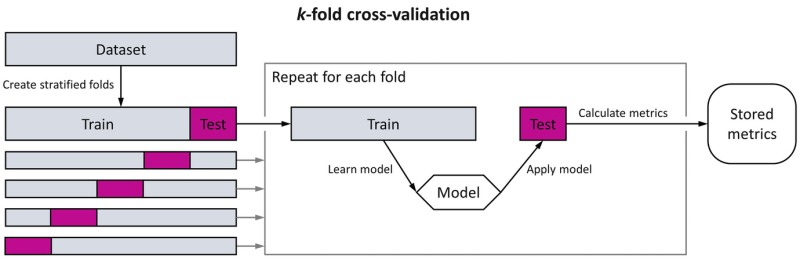
\includegraphics[width=6.06111in,height=2.68611in]{img/analisis de metodologia/463627_1_En_8_Fig8_HTML.jpg}
  \caption{Flujo gráfico Tecnicas convinadas Stratified K-Fold CV}
  \label{fig:flujo_kfoldcvstratfield}
\end{figure}
